\section{Experimental Evaluation}

\subsection{Experimental Setup}

% \begin{table}[htbp]
%  \caption{Benchmarks categorization~\cite{bienia08characterization,woo1995splash,southern2016analysis}}
%  \center
%  \label{BC}
%   \scalebox{1}{
%   \begin{tabular}{ p{2.1cm} |  p{1.6cm} | p{1.6cm} | p{1.4cm} }
%     \hline
%    Name & Sync. Rate & Comm/Comp Ratio & No. Threads\\
%    \hline
%    blackscholes &  low & high & 1 + n \\
%    bodytrack &  medium & high & 2 + n\\
%    dedup &  medium & high & 3 + 3n\\
%    ferret &  high & medium & 3 + 4n\\
%    fluidanimate &  very high & low & 1 + n\\
%    freqmine &  high & high & n\\
%    swaptions &  low & low & 1 + n\\
%    radix &  low & high & n\\
%    lu\_ncb & low & low & n \\
%    lu\_cb &  low & low & n\\
%    ocean\_cp &  low & low & n\\
%    water\_nsquared &  medium & medium & n\\
%    water\_spatial &  low & low & n\\
%    fmm &  medium & low & n\\
%    fft &  low & high & n\\
%    \hline
%    % \bottomrule
%  \end{tabular}}
%\end{table}

% VJ: OLD VERSION
%\textbf{\textit{Experimental Environment:}} We ran our experiments on GEM5, simulating an ARM big.LITTLE-like architecture. The big cores are similar to out-of-order 2 GHz CortexA57 cores, with a 48 KB L1 instruction cache, a 32 KB L1 data cache, and a 2 MB L2 cache. The little cores are similar to in-order 1.2 GHz CortexA53 ones, with a 32 KB L1 instruction cache, a 32 KB L1 data cache, and a 512 KB L2 cache. We evaluated four distinct hardware configurations: 2B2S,2B4S,4B2S,4B4S, where B denotes big cores and S denoted little cores.
%%Two had balanced numbers of big and little cores, one with two big and two little cores (2B2S) and one with four big and four little ones (4B4S). The other two had different numbers of big and little cores, one with two big and four little cores (2B4S) and one with four big cores and two little cores (4B2S). 
%The OS is Linux v3.16. We cross-compiled the kernel with gcc v5.4.0, while we compiled the benchmarks inside the emulated environment with gcc v4.8.2.
%We chose to use a simulated environment to make it easier to evaluate our approach on multiple different hardware configurations. While we targeted simulated ARM cores, the underlying general procedure and model can be implemented on any real processor as long as they provide enough hardware performance monitor units (PMU). All hardware counters used by our model are supported by the real ARM Cortex-A57/A53 \cite{ARMA57} PMU.

\textbf{\textit{Experimental Environment:}} We first ran our experiments on GEM5, simulating an ARM big.LITTLE-like architecture. The big cores are similar to out-of-order 2 GHz CortexA57 cores, with a 48 KB L1 instruction cache, 32 KB L1 data cache and 2 MB L2 cache. The little cores are similar to in-order 1.2 GHz CortexA53 ones, with a 32 KB L1 instruction cache, 32 KB L1 data cache and 512 KB L2 cache. We evaluated four distinct hardware configurations on GEM5: 2B2S, 2B4S, 4B2S, 4B4S, where B denotes big cores and S denoted little cores.
%%Two had balanced numbers of big and little cores, one with two big and two little cores (2B2S) and one with four big and four little ones (4B4S). The other two had different numbers of big and little cores, one with two big and four little cores (2B4S) and one with four big cores and two little cores (4B2S). 
% VJ : I would get rid of the OS and compiler version...Unless it matters which kernel we are using
%The OS is Linux v3.16. We cross-compiled the kernel with gcc v5.4.0, while we compiled the benchmarks inside the emulated environment with gcc v4.8.2.
%We chose to use a simulated environment to make it easier to evaluate our approach on multiple different hardware configurations.
%While we targeted simulated ARM cores, the underlying general procedure and model can be implemented on any real processor as long as they provide enough hardware performance monitor units (PMU). All hardware counters used by our model are supported by the real ARM Cortex-A57/A53 \cite{ARMA57} PMU.
We then validate COLAB and its energy-aware extension on a HiHope Hikey 970 development board with 4 Cortex-A73 big cores at 2.36GHz and 4 Cortex-A53 little cores at 1.8GHz. As there is only 4 big cores in total to produce baseline performance, we evaluate four configurations: 1B1S, 1B3S, 2B2S and 3B1S. 

 \begin{table}[htbp]
  \caption{Benchmarks categorization~\cite{bienia08characterization,woo1995splash,southern2016analysis}}
  \center
  \label{BC}
   \scalebox{1}{
   \begin{tabular}{ p{2.5cm} |  p{2.0cm} | p{3cm} }
     \hline
     Name & Sync. Rate & Comm/Comp Ratio\\
    \hline
    blackscholes &  low & high \\
    bodytrack &  medium & high \\
    dedup &  medium & high \\
    ferret &  high & medium \\
    fluidanimate &  very high & low \\
    freqmine &  high & high \\
    swaptions &  low & low \\
    radix &  low & high \\
    lu\_ncb & low & low \\
    lu\_cb &  low & low \\
    ocean\_cp &  low & low \\
    water\_nsquared &  medium & medium \\
    water\_spatial &  low & low \\
    fmm &  medium & low \\
    fft &  low & high \\
    \hline
    % \bottomrule
  \end{tabular}}
\end{table}


 \begin{table*}
  \caption{Multi-programmed Workloads Compositions}
  \center
  \label{WC}
   \scalebox{0.9}{
   \begin{tabular}{ p{2cm} | p{7cm} | p{4cm} | p{2cm} }
    \hline
     \multicolumn{4}{c}{Synchronization-intensive VS Non-synchronization-intensive Workloads}\\
    \hline
     Index & Workload Composition & Synchronizations & Threads \\
    \hline
    Sync - 1 & water\_nsquared - fmm & intensive & 4 \\
    Sync - 2 & dedup - fluidanimate & intensive & 18 \\
    Sync - 3 & water\_nsquared - fmm - fluidanimate - bodytrack & intensive & 9 \\
    Sync - 4 & dedup - ferret - fmm - water\_nsquared & intensive & 20\\
    \hline
    NSync - 1 & water\_spatial - lu\_cb & non-intensive & 4 \\
    NSync - 2 & blackscholes - swaptions & non-intensive & 16 \\
    NSync - 3 & radix - fft - water\_spatial - lu\_cb & non-intensive & 8\\
    NSync - 4 & blackscholes - ocean\_cp - lu\_ncb - swaptions & non-intensive & 20\\
     \hline
     \multicolumn{4}{c}{Communication-intensive VS Computation-intensive Workloads}\\
     \hline
     Index & Workload Composition & Comm/Comp & Threads \\
    \hline
    Comm - 1 & water\_nsquared - blackscholes & Communication-intensive & 4 \\
    Comm - 2 & ferret - dedup &  Communication-intensive & 16 \\
    Comm - 3 & water\_nsquared - fft - radix - bodytrack &  Communication-intensive & 9 \\
    Comm - 4 & blackscholes - dedup - ferret - water\_nsquared &  Communication-intensive & 20\\
    \hline
    Comp - 1 & water\_spatial - fmm & Computation-intensive & 4 \\
    Comp - 2 & fluidanimate - swaptions & Computation-intensive & 17 \\
    Comp - 3 & lu\_ncb - fmm - water\_spatial - lu\_cb & Computation-intensive & 8\\
    Comp - 4 & fluidanimate - ocean\_cp - lu\_ncb - swaptions & Computation-intensive & 20\\
    \hline
      \end{tabular}}
  \scalebox{0.8}{
  \begin{tabular}{p{1.5cm} |p{4cm} |p{1cm}|| p{1.5cm} |p{7cm} |p{1cm}}
    \multicolumn{6}{c}{Large Mixed Multi-programmed Workloads for Real System Validation}\\
    \hline
   Index & Workload Composition & Threads & Index & Workload Composition & Threads\\
    \hline
    Large - 1 & radix - ocean\_cp & 5 & Large - 3 & blackscholes - radix - fluidanimate - water\_spatial & 15\\
    Large - 2 & ferret - swaptions & 24 & Large - 4 & ocean\_cp - ferret - lu\_cb - swaptions & 29\\
    \hline
  \end{tabular}}
\end{table*}

\begin{comment}
  \scalebox{0.8}{
  \begin{tabular}{p{1.5cm} |p{4cm} |p{1cm}|| p{1.5cm} |p{7cm} |p{1cm}}
   \hline 
  \multicolumn{6}{c}{Random-mixed Multi-programmed Workloads}\\
  \hline
      Index & Workload Composition & Threads & Index & Workload Composition & Threads\\
   \hline
    Rand - 1 &lu\_cb - dedup & 19& Rand - 6 &water\_spatial - fmm - fft - fluidanimate &21\\
    Rand - 2 &lu\_ncb - bodytrack &10& Rand - 7 &fmm - water\_spatial - ferret - swaptions&20\\
    Rand - 3 &ferret - water\_spatial&9 & Rand - 8 &water\_spatial - water\_nsquared - ferret - freqmine&17\\
    Rand - 4 &ocean\_cp - fft&8 & Rand - 9 &blackscholes - bodytrack - dedup - fluidanimate&55\\
    Rand - 5 &freqmine - water\_nsquared&6 & Rand - 10 &lu\_cb - lu\_ncb - bodytrack - dedup&53\\
   \hline
  \end{tabular}}
%\end{table*}
\end{comment}

\textbf{\textit{Workloads:}} For our workloads we used 15 different benchmarks (Table~\ref{BC}), pulled from PARSEC3.0~\cite{bienia11benchmarking} and SPLASH2~\cite{woo1995splash}.
%\footnote{Our version of GEM5 cannot simulate all PARSEC3.0 benchmarks on ARM. On top of \emph{canneal} and \emph{raytrace} that other researchers have also failed to build~\cite{endo2014micro,van2013full}. Among the SPLASH2 benchmarks, \emph{cholesky} and \emph{volrend} depended on huge input data files that did not fit on the hard drive image. We could not use \emph{barnes}, \emph{radiosity}, \emph{facesim}, \emph{x264}, \emph{vips} and \emph{streamcluster} because their runtime is prohibitively long even for $simsmall$ inputs.}
We only use the \emph{simsmall} inputs on GEM5 as it is well-known that the simulation is extremely slow. We group the benchmarks based on two criteria: a) synchronization intensity and b) communication vs computation intensity.
For each group, we randomly generate workloads with variable numbers of benchmarks and threads. These workloads allow us to investigate the behavior of the three scheduling policies under different extremes.
We then use large mixed workloads with the \emph{simlarge} inputs on  HiHope  Hikey  970 to explore the general  cases and validate COLAB with its energy-aware extension on the real chip with asymmetric multi-core processors.
Table~\ref{WC} shows the selected workloads. 

%For all of them, the experiment starts from a checkpoint taken after all benchmarks have completed their initialization.

%Each individual result represents the average over two simulations with different core orders - either big cores first or little cores first. Even small variations in the initial state of the system can have a significant effect on scheduling decisions and thus performance. For the Linux scheduler in particular, the order of starting benchmarks will decide which benchmarks will be initially assigned to big and little cores. By varying the initial state and measuring average runtimes over multiple simulations, we minimize the effect of randomness on our evaluation.

\textbf{\textit{Performance Metrics:}} Our evaluation uses two metrics to quantify scheduling efficiency: {\it Heterogeneous Average Normalized Turnaround Time} (H\_ANTT) and {\it Heterogeneous System Throughput} (H\_STP). They are based on ANTT and STP, as introduced in~\cite{eyerman2008system}. Both ANTT and STP use as their baseline the runtime of each application when executed on its own, i.e. when there is no resource sharing and scheduling decisions have little effect. ANTT is the average slowdown of all applications in the mix relative to their isolated baseline runtime. STP is the sum of the throughputs of all applications, relative to their isolated throughput.

For AMPs, these two metrics fail to work as intended. The runtime when executed alone is still affected by scheduling decisions, e.g. which threads to run on big cores. To overcome the problem, our modified metrics H\_ANTT and H\_STP use the runtime of each application in the mix when executed alone \emph{on a system where there are only big cores}. If the turnaround time of each application $i$ while being co-scheduled is $T^{M}_i$ and the turnaround time for the same application when running alone on a big-only system is $T^{SB}_i$, then:
$$ H\_ANTT = \frac{1}{n}\sum^{n}_{i=1}\frac{T^{M}_i}{T^{SB}_i}
,\ \ H\_STP = \sum^{n}_{i=1}\frac{T^{SB}_i}{T^{M}_i}$$
%When we evaluate a single benchmark on its own, we use the {\it Heterogeneous Normalized Turnaround Time} (H\_NTT):
%$$ H\_NTT = \frac{T^{M}}{T^{SB}}$$
H\_ANTT is better when lower, H\_STP is better when higher. For most figures, we further normalize our results relative to the Linux CFS results for the same configuration and workload.

\textbf{\textit{Schedulers:}}
We evaluate COLAB by comparing it against the default Linux CFS scheduler~\cite{molnar2007cfs} and a state-of-the-art realistic scheduler based on WASH~\cite{jibaja2016portable}. 
Linux CFS is the default scheduler on the GEM5 simulator and ARM GTS~\cite{jeff2013big} is the default scheduler on the development board. They provide fairness while trying to maximize the overall CPU resource utilization.
%The original WASH was implemented inside a Java VM to control Java thread affinities.
%In our re-implementation of WASH, we use the same heuristic but we drive it with a core sensitivity model that fits the simulated system and we use it for controlling all application threads. 

%\begin{figure}
%\centering
%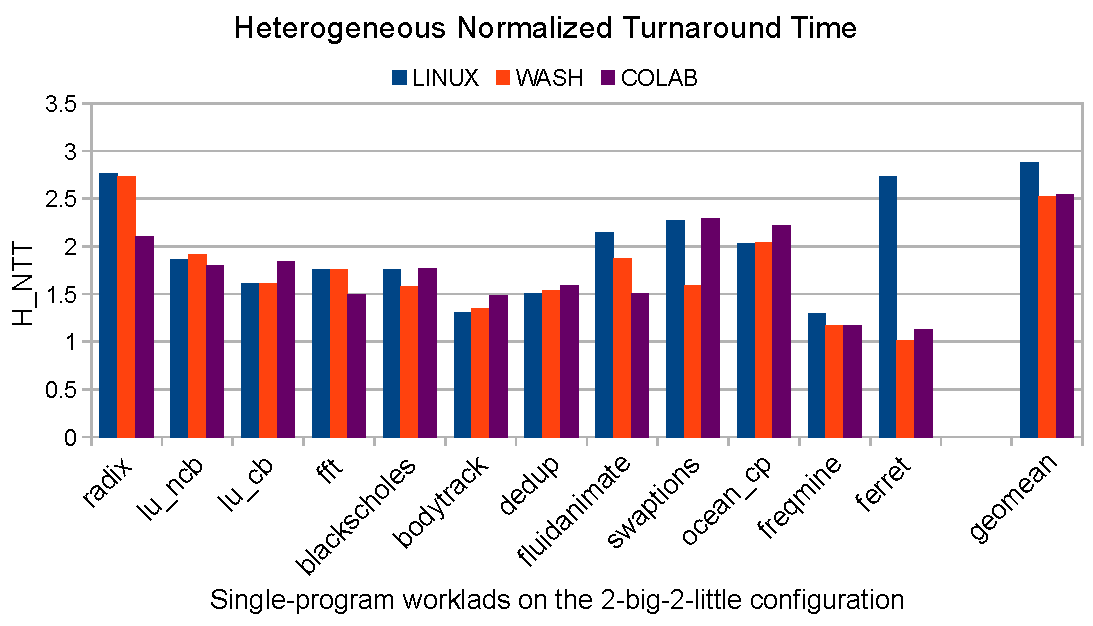
\includegraphics[scale=0.48]{figures/MSW2.pdf}
%\caption{Performance of single program workloads on a 2-big 2-little system. Lower is better.}
%\label{MSW}
%\end{figure}  

%\subsection{Single-programmed Workloads}
%Much of the research on AMP scheduling focuses on single-programmed workloads, where fairness and load balancing are not important and the focus is on core sensitivity and bottleneck acceleration. In this section, we examine how COLAB fares under this scenario. Figure~\ref{MSW} shows H\_NTT under Linux (blue), WASH (red) and COLAB (violet), for our multi-threaded benchmarks when executed alone on a 2-big-2-little hardware configuration. 
%We do not consider the three SPLASH2 benchmarks \emph{fmm}, \emph{water\_nsquared} and \emph{water\_spatial}, since they do not support more than 2 threads with $simsmall$ input size on GEM5 and scheduling them optimally for performance is trivial.

%The AMP-agnostic Linux scheduler is inappropriate for most benchmarks. COLAB improves H\_NTT by up to 58\% and by 12\% on average and up to 173\% over Linux CFS for \emph{ferret}, where most computation happens in a pipeline pattern with unbalanced stages. AMP-aware schedulers take advantage of that by scheduling the longest stages, the bottleneck threads, on big cores. As a result, COLAB does only 13\% worse than running on a system \emph{with four big cores}.
%Compared to WASH, COLAB achieves its best result for \emph{fluidanimate}. Previous work~\cite{bienia08characterization} has shown that \emph{fluidanimate} has around 100x more lock-based synchronizations than other PARSEC applications. Our collaborative core allocation and thread selection policy is much better than WASH at prioritizing bottleneck threads.  As a result, we reduce turnaround time by 30\% compared to Linux and 20\% compared to WASH.
%In some cases, such as \emph{bodytrack}, \emph{lu\_ncb}, or \emph{freqmine}, AMP-awareness has little effect on performance. Such benchmarks split work dynamically between threads, which then all have the same core sensitivity and the application adapts automatically to asymmetries in processing speed. AMP-aware policies offer no benefit while introducing overheads, as was also noted in~\cite{jibaja2016portable}. The pipeline benchmark \emph{dedup} has five stages to stream the input set. When there are more threads than available cores, both heterogeneous-aware schedulers can not service the excess threads in time, resulting in a certain impact on overall system performance.
%There is only one case where COLAB performs significantly worse than WASH. For \emph{swaptions}, we perform as well as the AMP-agnostic Linux scheduler while WASH improves turnaround time by 31\%. This is because the bottleneck threads of \emph{swaptions} are core insensitive while the non-bottleneck threads are core sensitive. This being the ideal case for WASH, it improves turnaround time while we fail to do the same.

%On average, WASH and COLAB perform similarly well and improve performance by 12\% compared to Linux when handling single program workloads. This is a limited scenario, with no need for fairness and a simple decision space. COLAB was not expected to perform much better than the state-of-the-art, doing as well as it is a positive result.
%\vspace{-1.2em}
\subsection{Experiments on GEM5}
%\vspace{-0.3cm}
In this section, we evaluate the performance of COLAB under multi-threaded multi-programmed workloads on the GEM5 simulator. Overall, our scheduler is able to outperform both the Linux CFS and WASH when there is room for improvement. This is particularly true when we have a limited number of big cores and/or many communication-intensive benchmarks. In such cases, we need to consider \emph{at the same time} both core affinity and thread bottlenecks. COLAB can do that, while CFS and WASH cannot, leading to significant performance improvements. In the rest of this subsection, we examine the behavior of COLAB under four different hardware configurations
%(2B2S, 2B4S, 4B2S, 4B4S) 
for the five different classes of workloads shown in Table~\ref{WC}.

\begin{figure}
\centering
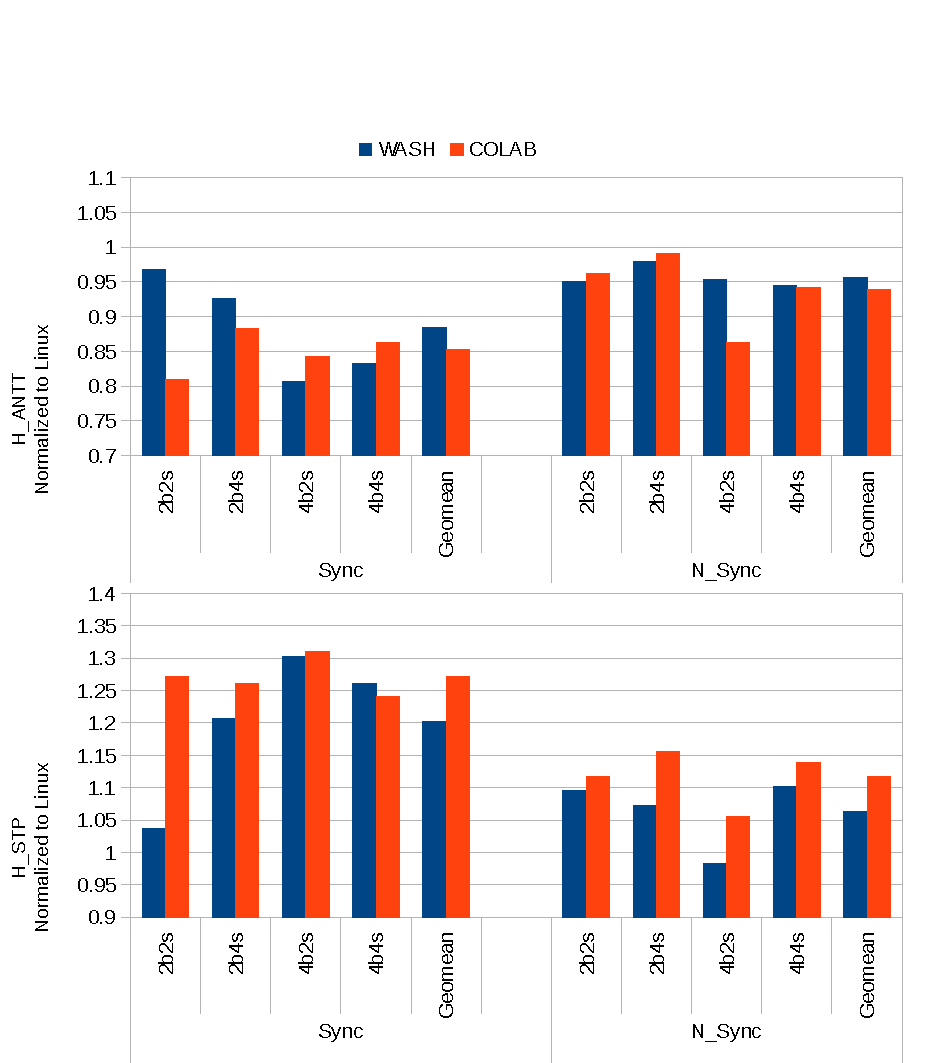
\includegraphics[scale=0.55]{figures/sync.pdf}
%\caption{Heterogeneous Average Normalized Turnaround Time (H\_ANTT) and Heterogeneous System Throughput (H\_STP) 
\caption{Performance of Synchronization-Intensive and Non-Synchronization-Intensive Workloads. All results are normalized to the Linux CFS ones. Lower is better for H\_ANTT and higher is better for H\_STP.}
\label{sync}
\end{figure} 

\textbf{\textit{Synchronization-intensive vs Synchronization Non-intensive workloads:}}
The synchronization-intensive group contains workloads where all programs have high synchronization rates. Because of this, we expect them to have a large number of bottleneck threads, so COLAB should be able to schedule them better than CFS and WASH. Conversely, synchronization non-intensive workloads should provide few opportunities for COLAB to improve on CFS and WASH.

Figure~\ref{sync} show the performance of all three schedulers for each workload class and hardware configuration. The two plots show the 
average H\_ANTT (top) and the average H\_STP (bottom). The left and right half of each plot contain the results for the synchronization-intensive (\emph{Sync}) and synchronization non-intensive (\emph{N\_Sync}) workload classes, respectively.
The results agree with our expectations. We observe that COLAB improves the turnaround time of \emph{Sync} workloads by around 15\% and 4\% on average compared to CFS and WASH, respectively. We also see that hardware configurations with low core counts, such as 2B2S, favor COLAB. We reduce turnaround time by up to 20\% over CFS and by up to 16\% over WASH. With fewer cores, the pressure from co-executed applications rises and properly balancing bottleneck acceleration and core sensitivity across multiple programs becomes increasingly difficult. WASH places all bottleneck threads onto the big cores, which results in these threads having to wait for CPU time in busy run queues, ending up with only 3\% of performance improvement over Linux. COLAB handles these bottleneck threads in a more holistic way, improving turnaround time by 20\% and system throughput by 27\%, compared to Linux.

As for \emph{N\_Sync} workloads, there are few bottleneck threads to be accelerated, making scheduling decisions much easier. As a result, both COLAB and WASH perform similarly to Linux, with COLAB improving average turnaround time by 6\% and average system throughput by 12\% compared to Linux.
An interesting point is that COLAB does significantly better (10\% and 15\% improvement on turnaround time) than WASH and Linux for \emph{N\_Sync} workloads on the 4B2S configuration. In this case, where we have sufficient big core resources without enough critical threads, WASH keeps migrating predicted critical threads on big cores even when there is no actual need. However, COLAB will make intelligent decisions by keeping relatively more threads on little cores, which gives more chance for big cores to always execute the limited \emph{really critical} threads as soon as possible.
% (PP: Turnaround time is worse for COLAB. Unless we go into details about why turnaround time is worse while throughput is better, saying that we do slightly better is wrong. Also it would be nice for the previous paragraph to identify the specific workloads which are accelerated more and pinpoint what makes COLAB better in this case.) 
%This also explains why WASH does slightly better than COLAB on 2B4S configuration for these workloads - When there are not enough critical threads to be accelerated, the low big-to-little ratio could guide the WASH to migrate less threads on big cores while COLAB does not sensitive to this ratio. 

\begin{figure}
\centering
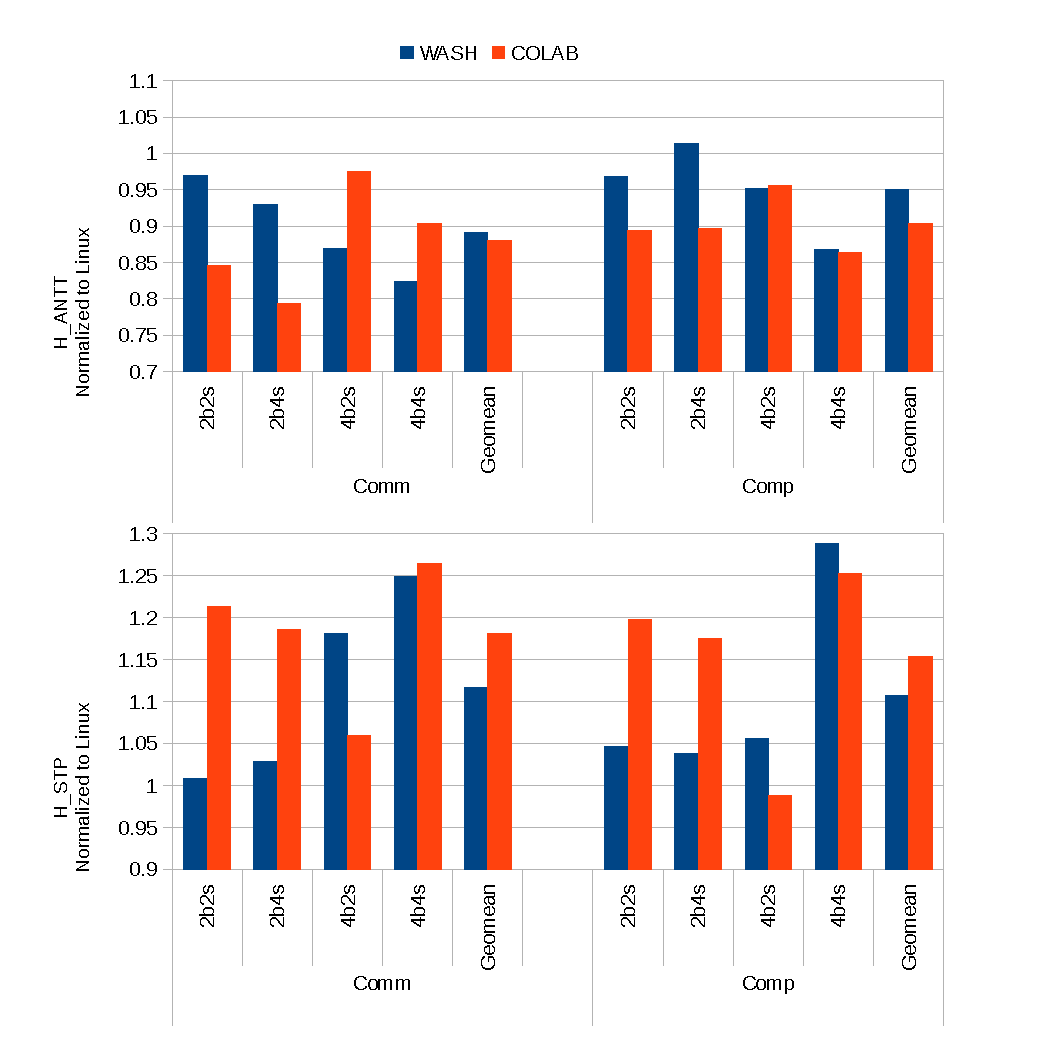
\includegraphics[scale=0.55]{figures/com.pdf}
%\caption{Heterogeneous Average Normalized Turnaround Time (H\_ANTT) and Heterogeneous System Throughput (H\_STP)
\vspace{-0.35cm}
\caption{Performance of Communication-Intensive and Computation-Intensive Workloads. All results are normalized to the Linux CFS ones. Lower is better for H\_ANTT and higher is better for H\_STP.}
\label{com}
\end{figure} 

\textbf{\textit{Communication-intensive vs Computation-intensive workloads:}}
When handling programs with high communication-to-computation ratios, bottleneck threads are likely to arise and accelerating them is critical. This is an ideal scenario for COLAB. On the other hand, workloads with little communication are easier to schedule, so CFS and WASH should do reasonably well, leaving little space for improvement.

Figure~\ref{com} shows the evaluation results for these two classes of workloads, \emph{Comm} and \emph{Comp}. Both COLAB and WASH improve over the Linux scheduler for communication-intensive workloads. They, however, offer different advantages on different hardware configurations. COLAB distributes the bottleneck threads to both big and little cores which is extremely important when having only two big cores (2B2S, 2B4S). COLAB improves the turnaround time by up to 21\% compared to Linux and 15\% compared to WASH on the 2B4S configuration. When more big cores are available, WASH does better as it keeps all bottleneck threads on big cores. On these configurations, WASH improves turnaround time by up to 18\% over Linux (on the 4B4S configuration) and up to 10\% over COLAB (on the 4B2S configuration). On average, COLAB reduces turnaround time by around 12\% compared to Linux and 1\% compared to WASH for the communication-intensive workload class.
Figure~\ref{com} also confirms that there are few opportunities for better scheduling with computation-intensive workloads. Still, COLAB does better than WASH and Linux. Its turnaround time and system throughput are improved by around 10\% and 15\%, respectively, compared to Linux and 5\% compared to WASH. This is, again, due to a fact that multiple bottlenecks are distributed both to big and little cores, which results in more efficient use of the available hardware resources for the few bottlenecks that are present.

\begin{comment}
\begin{figure}
\centering
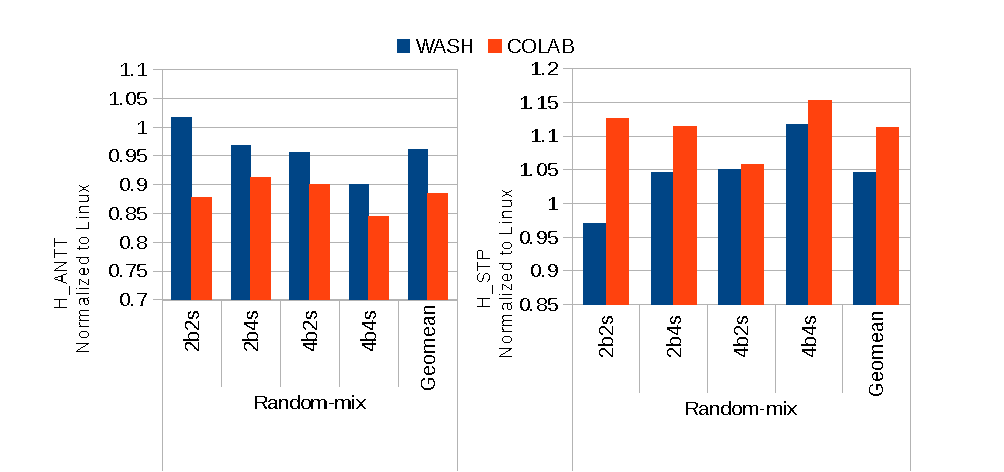
\includegraphics[scale=0.55]{figures/rand.pdf}
%\caption{Heterogeneous Average Normalized Turnaround Time (H\_ANTT) and Heterogeneous System Throughput (H\_STP)
\caption{Performance of 2- and 4-programmed Workloads. All results are normalized to the Linux CFS ones. Lower is better for H\_ANTT and higher is better for H\_STP.}
\label{rand}
\vspace{-0.2cm}
\end{figure} 
%\vspace{-1em}
\textbf{\textit{Mixed workloads:}}
This class of workloads represents the general case of different applications with different needs, affinities, and communication patterns competing for the same cores. Figure~\ref{rand} shows the results for 10 such workloads. COLAB performs very well for these workloads: more diverse programs mean more asymmetry, more bottlenecks, more critical threads, and more potential for acceleration. Our collaborative multi-factor scheduler carefully balancing all scheduling aims (core sensitivity, thread criticality and fairness) leads to a significant performance gain against WASH and Linux. COLAB improves turnaround time and system throughput by around 12\% and 11\% compared to Linux and around 8\% and 7\% compared to WASH.
\end{comment}
%\vspace{-1em}
\begin{figure}
\centering
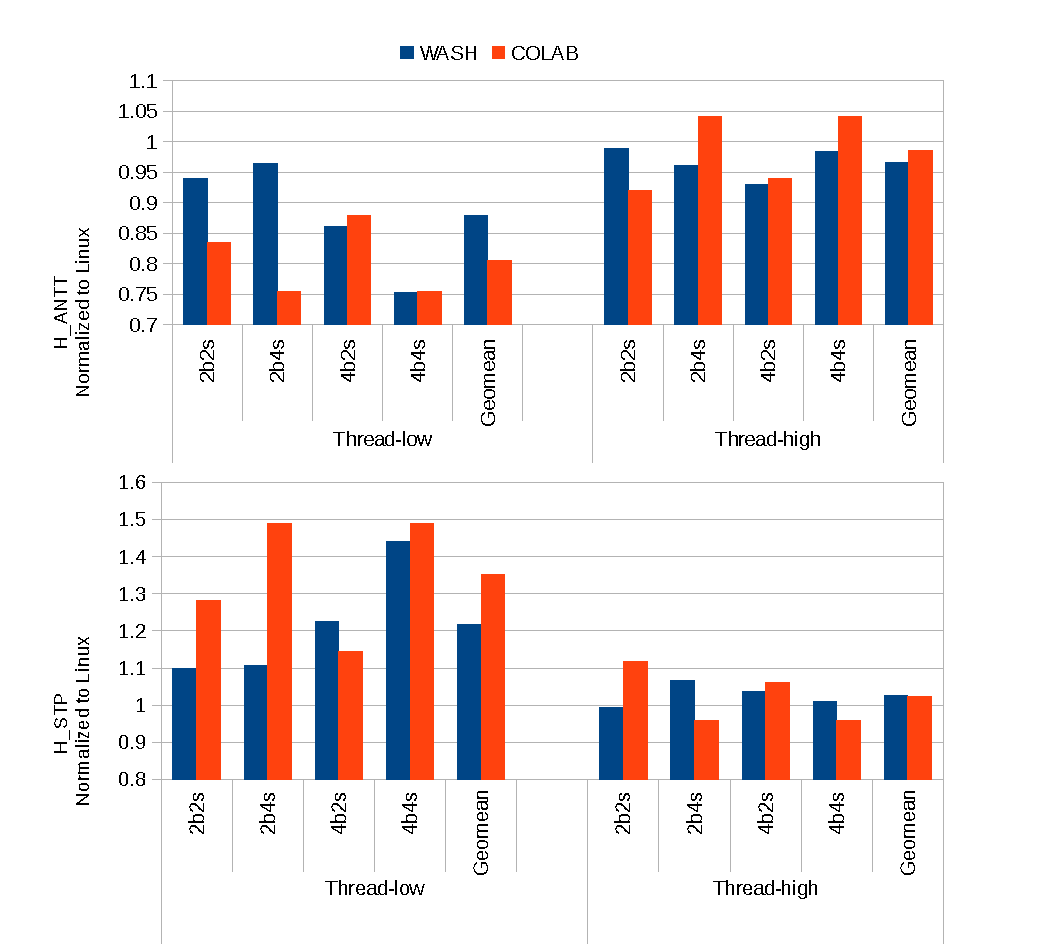
\includegraphics[scale=0.55]{figures/nthread.pdf}
%\caption{Heterogeneous Average Normalized Turnaround Time (H\_ANTT) and Heterogeneous System Throughput (H\_STP) 
\caption{Performance of low number of application threads and high number of application threads Workloads. All results are normalized to the Linux CFS ones. Lower is better for H\_ANTT and higher is better for H\_STP.}
\label{nthread}
\end{figure}
%\vspace{-1em}

\begin{figure}
\centering
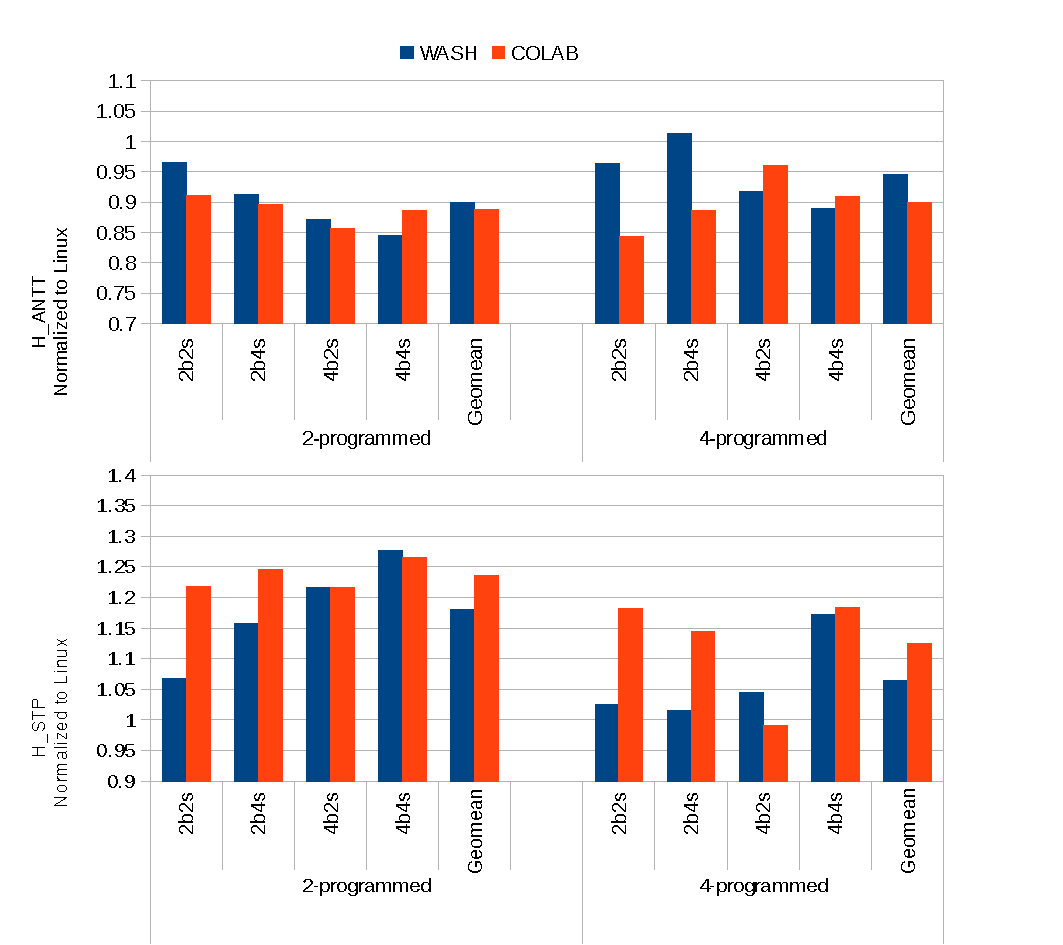
\includegraphics[scale=0.55]{figures/nprog.pdf}
%\caption{Heterogeneous Average Normalized Turnaround Time (H\_ANTT) and Heterogeneous System Throughput (H\_STP)
\caption{Performance of 2- and 4-programmed Workloads. All results are normalized to the Linux CFS ones. Lower is better for H\_ANTT and higher is better for H\_STP.}
\label{nprog}
\end{figure}
%\vspace{-1em}
%\begin{figure*}
%\centering
%\includegraphics[scale=0.6]{figures/all.png}
%\caption{Heterogeneous Average Normalized Turnaround Time (H\_ANTT) and Heterogeneous System Throughput (H\_STP)of multiprogrammed workloads averaged by different configurations. All results are normalized to the Linux CFS ones.}
%\label{M24W}
%\end{figure*}
\textbf{\textit{Thread and program count:}}
To examine the impact of thread and program count on the behavior of each scheduler, we grouped our experimental results based on these two properties. Figure~\ref{nthread} shows the performance of all schedulers both for workloads with a low thread count (less than the core count for that hardware configuration) and for workloads with a high thread count (at least double higher than the maximum core count). We observe that both COLAB and WASH perform significantly better than Linux for workloads with a low number of threads. Fewer threads make it easier to identify bottleneck threads and give them the resources they need - either by migrating them to big cores (WASH and COLAB) or by prioritizing them on little cores (COLAB). With limited big core resources, COLAB does much better than WASH since it distributes bottleneck threads on all available cores, avoiding overloading the few big cores and keeping the little cores idle. COLAB outperforms Linux by up to 25\% (2B4S) and WASH by up to 21\% (2B4S) on turnaround time. On average, COLAB improves turnaround time and system throughput by around 20\% and 35\% compared to Linux and around 8\% and 11\% compared to WASH for workloads with a low number of threads.
For workloads with a high thread count, neither Linux nor WASH are able to improve much on Linux. Overloading the system with threads means that, regardless of where we place threads, cores will have long runqueues. 
In this case, all cores will have long run queues and COLAB and WASH increase the management overhead (including more frequent thread migrations) with little benefit, leading to performance degradation. Of the two heterogeneity-aware schedulers, COLAB, with its scale-slice technique, more frequently migrates threads, which results in a slightly worse performance than WASH. On average, COLAB improves turnaround time and system throughput by less than 2\% and 3\% compared to Linux, while WASH slightly outperforms COLAB by 2\% on turnaround time and 0.2\% on system throughput.

We see a similar picture when we considered workloads with different number of programs in them. Figure~\ref{nprog} shows the performance of all schedulers for 2-programmed and 4-programmed workloads. As in the case of high and low thread counts, increasing the number of co-executed programs gives higher pressure on the scheduler, increasing the waiting time of threads in runqueues and reducing the direct benefit of migration between waiting threads. But more programs also cause more bottlenecks and provide new opportunities for co-acceleration instead of only increasing data-parallel threads. 
%. Heterogeneous aware schedulers generally enjoy better performance gain against Linux on workloads with less programs. Similar as the issue in the above comparisons for total number of threads, more programs with more threads increase the waiting list on runqueues and reduce the direct benefit of migrations between waiting programs/threads.
By intelligently distributing bottleneck threads from different programs between big and little cores, COLAB faces less problems than WASH from the pressure of increasing programs. 

As a result, both COLAB and WASH outperform Linux by more than 10\% on 2-programmed workloads on turnaround time and COLAB can keep the 10\% performance gain also on 4-programmed workloads, while WASH reduced to only have 5\% performance gain on 4-programmed workloads. As for system throughput, COLAB improves by 23\% and 12\% on 2-programmed and 4-programmed workloads compared to Linux while improves by 5\% and 6\% on 2-programmed and 4-programmed workloads compared to WASH. 
%\textbf{VJ: This is a bit counterintuitive. Why do we get better results for COLAB scheduler when we have more programs but not when we have more threads in a workload?}


%\begin{itemize}
%\item \textbf{Synchronisation-intensive} workloads comprise of the programs that have high synchronisation rate. Our hypothesis was that these workloads contain more bottleneck threads, due to intensive synchronisation between different threads, and that the mechanisms we developed in COLAB scheduler will schedule these threads in more optimal way, compared to Linux and WASH schedulers. On the other hand, \textbf{Synchronisation-Nonintensive} workloads comprise of the programs that have low synchronisation rate, hence giving less opportunities to the COLAB scheduler to improve on Linux and WASH schedulers. Therefore, for these workloads we expected to see less impact from COLAB.
%\item \textbf{Communication-intensive} workload comprise of the programs that have high communication-to-computation ratio. This result in high volume of communication between program threads, which furher results not only in more bottleneck threads, but also in low amount of computation done by some threads. This scenario gives more opportunities to COLAB for improved scheduling decisions, therefore our hypothesis was that for these workloads we will get better results than Linux and WASH. \textbf{Computation-intensive} workloads comprise of applications that have high computation-to-communication ratio. Due to less bottleneck threads and more similarity in terms of computation load of each thread, there are less opportunities for the COLAB scheduler here to improve on Linux and WASH, therefore we expected similar results between all three scheduler.
%\item \textbf{Mixed} workloads represent the most general workloads, comprising a mixture of synchronisation-intensive, synchronisation-nonintensive, communication-intensive and computation-intensive programs. The intention of using these workload is to observe how well COLAB performs in general setting, compared to Linux and WASH.
%\end{itemize}

%\begin{figure}
%\centering
%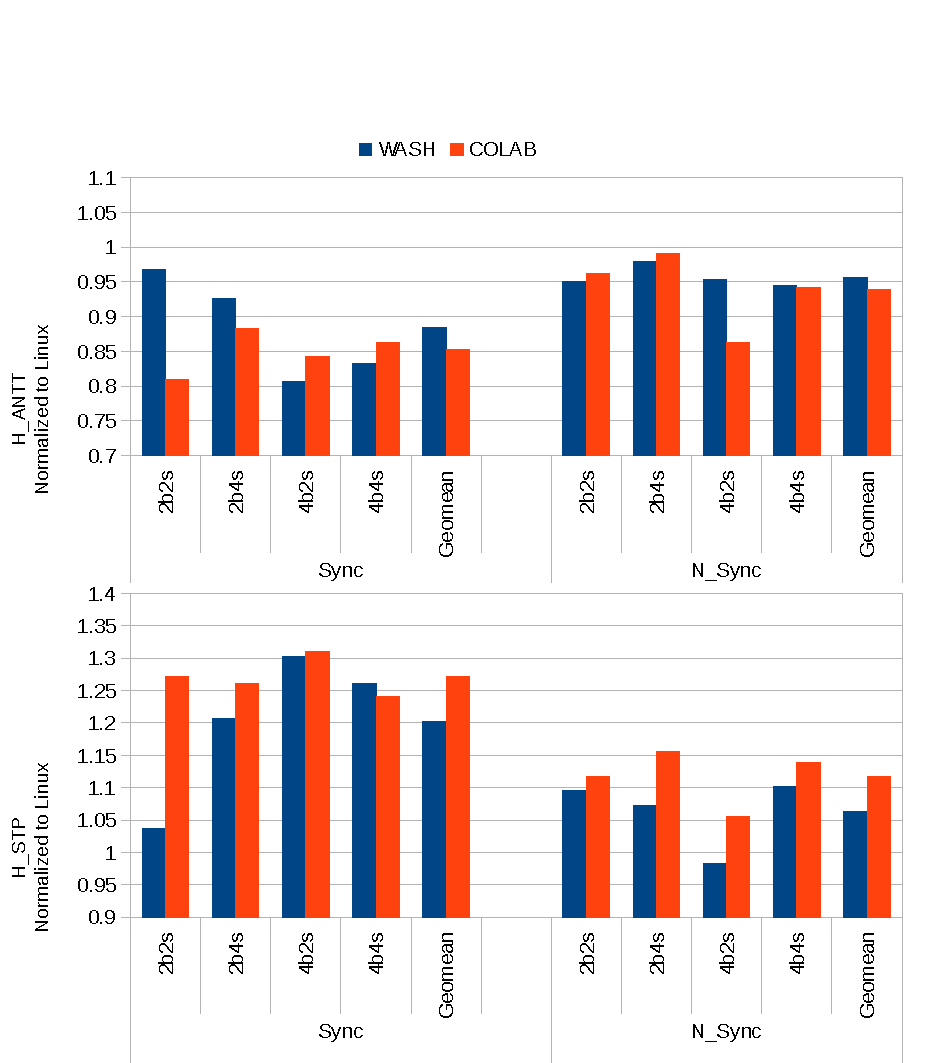
\includegraphics[scale=0.5]{figures/sync.pdf}
%\caption{Heterogeneous Average Normalized Turnaround Time (H\_ANTT) and Heterogeneous System Throughput (H\_STP) of Synchronization-Intensive and Non-Synchronization-Intensive Workloads. All results are normalized to the Linux CFS ones. Lower is better for H\_ANTT and higher is better for H\_STP.}
%\label{sync}
%\end{figure} 

%\paragraph{Synchronisation Intensive vs. Synchronisation Nonintensive Workloads} Figure~\ref{sync} shows the performances of all three schedulers on synchronization-intensive (\emph{Sync}) and synchronization-nonintensive (\emph{N\_Sync}) workloads. As with the other experiments in this section, the experiments here are grouped based on hardware configuration on which they are executed. We present the mean H\_ANTT and H\_STP over four different workloads.
%%(as shown in Figure~\ref{fig:XX}). Note again that lower H\_ANTT and higher H\_STP translate into higher performance of the scheduler. 
%We can observe that, for synchronisation-intensive workloads, COLAB improves turnaround time by around 15\% and 4\% on average compared to Linux and WASH, respectively. We can also observe that on the hardware configurations with smaller number of cores (2B2S), the COLAB scheduler performs especially well compared to Linux and WASH, improving over Linux by up to 20\% and over WASH by up to 16\%. Because Linux and WASH lack effective solutions to handle multiple threads of several applications accessing limited resources. With increasing  pressure  from  co-executed  applications, properly  balancing  bottleneck  acceleration and core sensitivity across multiple programs using only two big cores becomes difficult. WASH places all bottleneck threads onto the big cores, which results in these threads having to wait for CPU time in busy run queues, ending up with only 3\% of performance improvement over Linux. COLAB handles these bottleneck threads in a more holistic way, improving turnaround time by 20\% and system throughput by 27\%, compared to Linux.

%%Synchronization-intensive workloads fully composed by benchmarks with higher synchronization rates than others, which lead to the  much more importance of multiple bottlenecks and critical threads co-acceleration. Both heterogeneous-aware schedulers can show a significant advantage than Linux CFS on these cases. As a result, COLAB improves turnaround time by around 15\% compared to Linux and around 4\% compared to WASH on average of different configurations and workload compositions. On certain workloads and configuration cases, COLAB can outperform Linux by up to 20\% (2B2S) and outperform WASH by up to 16\% (2B2S). 
%%The state-of-the-art WASH scheduler shows its limitations when used on limited resources (2B2S). With increasing  pressure  from  co-executed  applications, properly  balancing  bottleneck  acceleration and core sensitivity across multiple programs using only two big cores becomes difficult. WASH identifies these bottlenecks and assigns their threads to big cores without further consideration. Instead of accelerating the bottleneck threads, this leads to the bottleneck threads getting stuck waiting for CPU time in busy runqueues. At the same time, non-critical threads enjoy short waiting times on little cores. WASH ends up performing only 3\% better than Linux CFS. COLAB handles bottleneck threads in a more holistic way, improving performance around 19\% for the same scenario.
%Similar results are presented for the system throughput. COLAB outperform Linux by around 27\% and outperform WASH by around 7\%. 

%As for synchronization-nonintensive workloads, neither COLAB nor WASH have a significant optimization space, since there are not enough bottleneck and critical threads that can be accelerated. As a result, both schedulers perform similarly to Linux, with COLAB improving turnaround time and system throughput by around 6\% and 12\% compared to Linux and around 2\% and 5\% compared to WASH. 
%\textbf{VJ: 12\% seems quite significant, though.} 

%\textit{This verifies our hypothesis that heterogeneity-aware schedulers bring more benefit, compared to the Linux scheduler, for workloads that are dominated by synchronisation-intensive programs. Furthermore, the COLAB scheduler notably outperforms the state-of-the-art WASH scheduler on limited-resource hardware configurations.}

%\begin{figure}
%\centering
%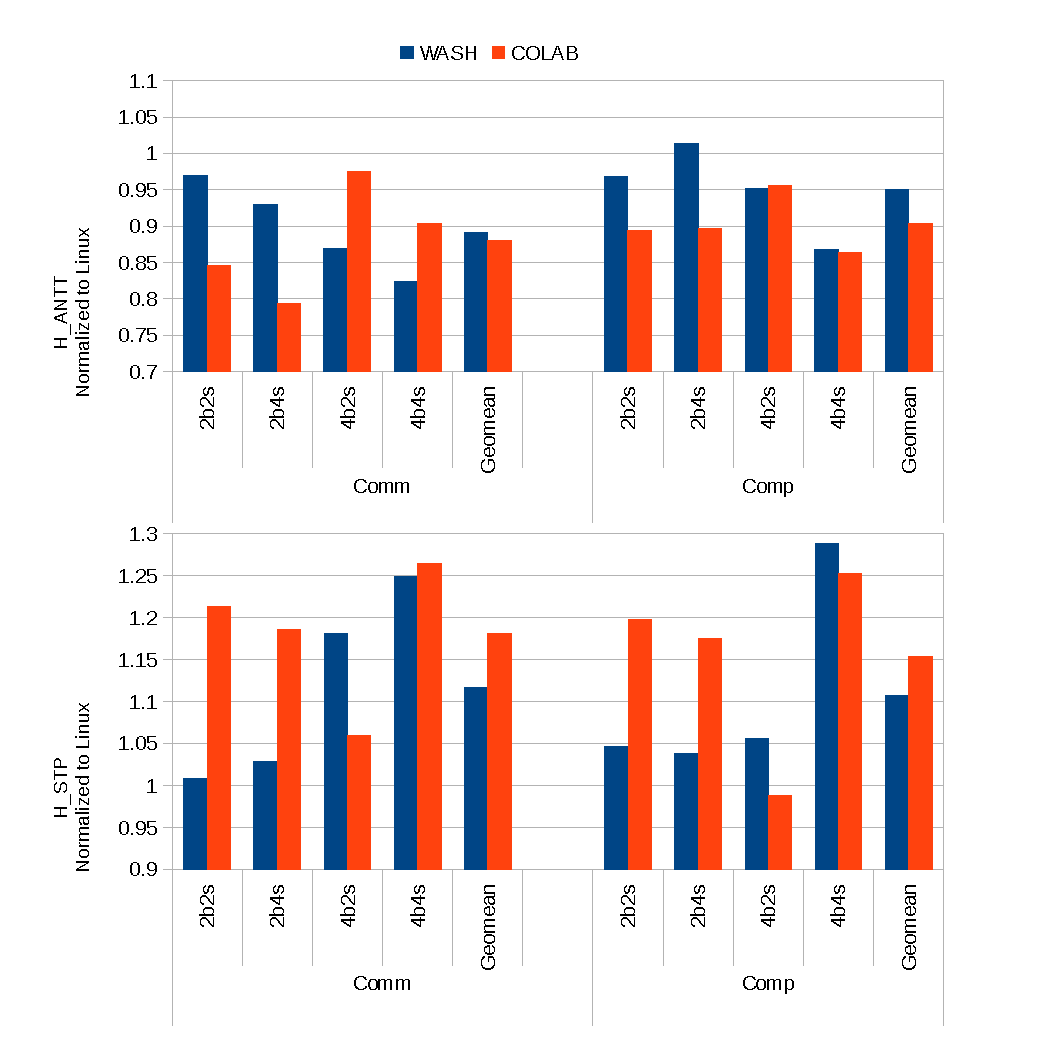
\includegraphics[scale=0.46]{figures/com.pdf}
%\caption{Heterogeneous Average Normalized Turnaround Time (H\_ANTT) and Heterogeneous System Throughput (H\_STP) of Communication-Intensive and Computation-Intensive Workloads. All results are normalized to the Linux CFS ones. Lower is better for H\_ANTT and higher is better for H\_STP.}
%\label{com}
%\end{figure} 

%\begin{figure}
%\centering
%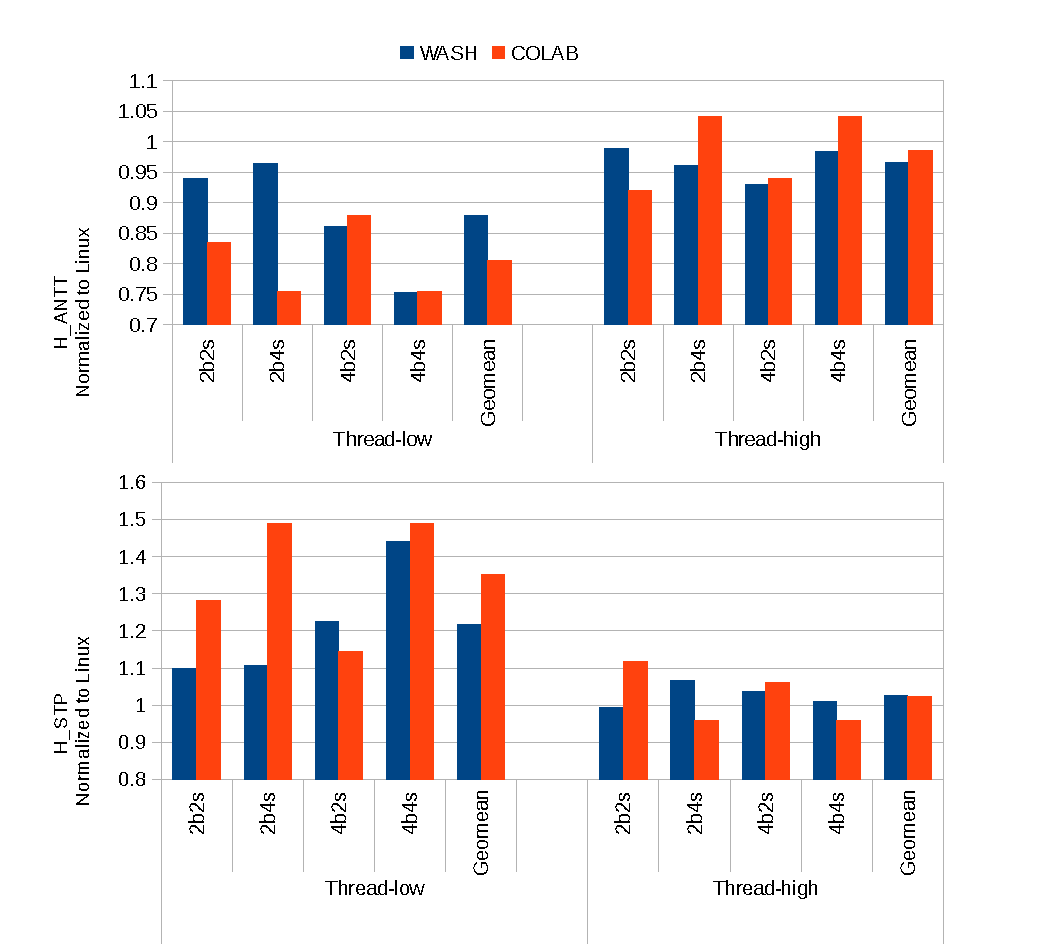
\includegraphics[scale=0.5]{figures/nthread.pdf}
%\caption{Heterogeneous Average Normalized Turnaround Time (H\_ANTT) and Heterogeneous System Throughput (H\_STP) of low number of application threads and high number of application threads Workloads. All results are normalized to the Linux CFS ones. Lower is better for H\_ANTT and higher is better for H\_STP.}
%\label{nthread}
%\end{figure} 

%\paragraph{Communication-intensive vs. Computation-intensive Workloads} Figure~\ref{com} shows the performance of COLAB, WASH and Linux schedulers on communication-intensive and computation-intensive workloads. 
%The hardware configuration is indicated on the X-axis of each subplot. Lower H\_ANTT and higher H\_STP translates into higher performance.
%Communication intensive workloads fully composed by benchmarks with high communication-to-computation ratio, which lead to a significant amount of intra-program communications between multiple application threads. This can result in not only multiple runtime bottlenecks, but also light computation of each thread. So multiple bottlenecks need to be co-executed and each of them has lighter computation need to be done.
%Both COLAB and WASH schedulers improve the Linux scheduler. They, however, offer different advantages on different hardware configurations. COLAB distributes the bottleneck threads to both big and little cores, which results in more significant improvements on limited big-core cases (2B2S, 2B4S). COLAB improves the turnaround time by up to 21\% compared to Linux and 15\% compared to COLAB on the 2B4S configuration. As is the case with the synchronisation-intensive workloads, WASH accumulates the bottleneck threads on big cores only, which results in a better performance where there are enough big-core cases (4B2S, 4B4S). On these configurations, WASH improves turnaround time by up to 18\% over Linux (on 4B4S configuration) and up to 10\% over COLAB (on 4B2S configuration). On average, COLAB improves the turnaround time by around 12\% compared to Linux and 1\% compared to WASH for the communication intensive workloads on all configurations. We observe similar results for system throughput, where COLAB outperforms Linux by around 18\% and outperforms WASH by around 5\%.

%As noted before, computation-intensive workloads offer less improvement space for both heterogeneity-aware schedulers over Limux. Still, we can observe better performance for COLAB than for WASH and Linux, with COLAB improving turnaround time and system throughput by around 10\% and 15\%, respectively, compared to Linux and 5\% compared to WASH. This is, again, due to a fact that multiple bottlenecks are distributed both to big and little cores, which results in more efficient use of the available hardware resources for the few bottlenecks that are present.

%\emph{To summarise, heterogeneous aware schedulers show better performance gain on communication-intensive workloads than on computation-intensive workloads. COLAB outperforms WASH on both workloads on average and shows more significant advantage on computation-intensive workloads. WASH only outperforms COLAB on communication-intensive workloads when there are enough high performance big cores available.}
%%up to 36\% (Comm-4 on 2B2S) and outperform WASH by up tp 24\% (Comm-3 on 2B4S) on turnaround time.



%\begin{figure}
%\centering
%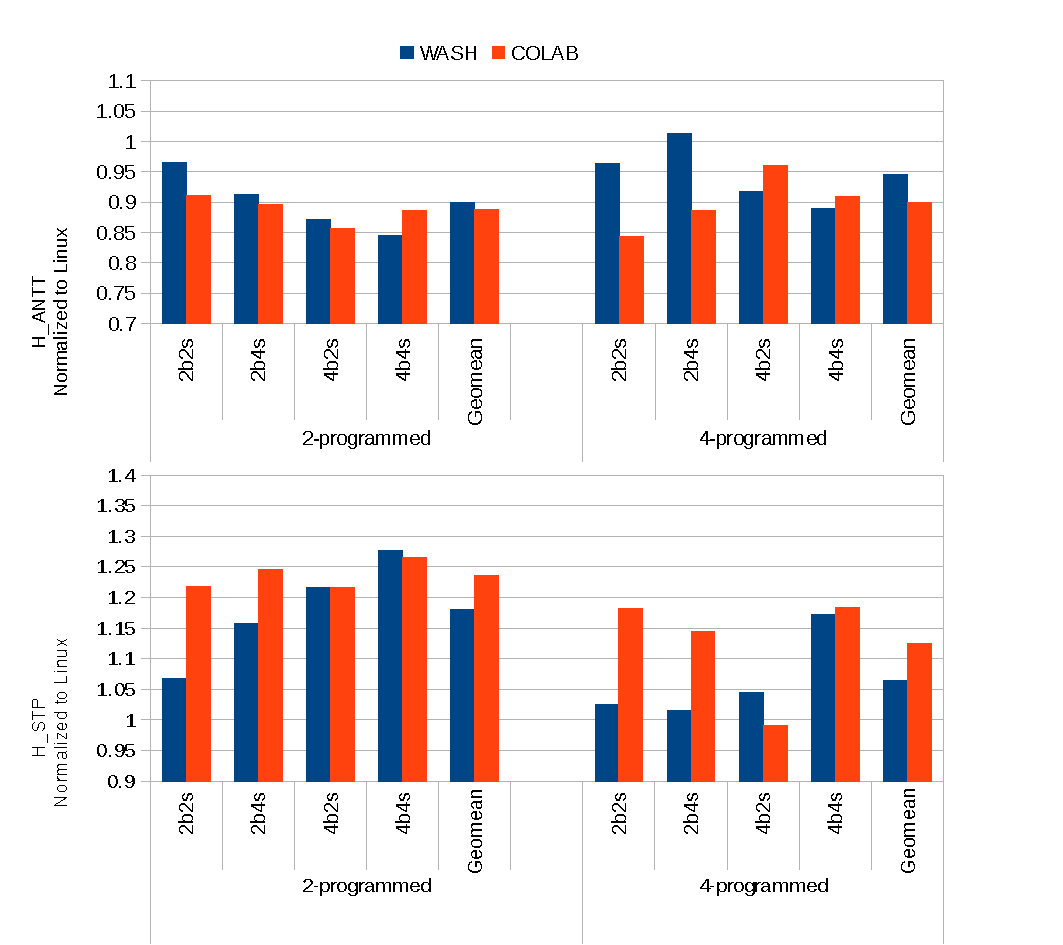
\includegraphics[scale=0.5]{figures/nprog.pdf}
%\caption{Heterogeneous Average Normalized Turnaround Time (H\_ANTT) and Heterogeneous System Throughput (H\_STP) of 2-programmed and 4-programmed Workloads. All results are normalized to the Linux CFS ones. Lower is better for H\_ANTT and higher is better for H\_STP.}
%\label{nprog}
%\end{figure} 

%\begin{figure*}
%\centering
%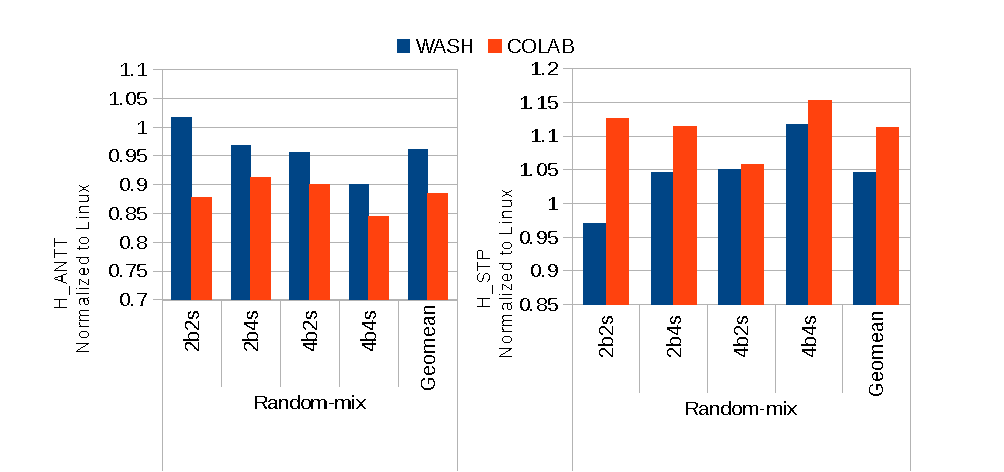
\includegraphics[scale=0.5]{figures/rand.png}
%\caption{Heterogeneous Average Normalized Turnaround Time (H\_ANTT) and Heterogeneous System Throughput (H\_STP) of 2-programmed and 4-programmed Workloads. All results are normalized to the Linux CFS ones. Lower is better for H\_ANTT and higher is better for H\_STP.}
%\label{rand}
%\end{figure*} 

%\paragraph{Mixed Workloads}
%Figure~\ref{rand} shows the performances of 10 mixed workloads. We can observe that COLAB performs very well for these workloads: more diverse programs mean more asymmetry, more bottlenecks, more type of critical threads and more potential for acceleration. Our collaborative multi-factor scheduler carefully handling all the issues (core sensitivity, thread criticality and fairness) brings a significant performance gain against WASH and Linux on this scenario - COLAB improves turnaround time and system throughput by around 12\% and 11\% compared to Linux and around 8\% and 7\% compared to WASH.

%\paragraph{Thread and program count} In our next set of experiments, we studied what impact does the total number of threads and a total number of programs in a workload has on the performance of heterogeneity-aware schedulers. Figure~\ref{nthread} shows the performance of all considered schedulers both for workloads comprising a low number of threads (where there is less threads than cores in the system) and for workloads comprising a high number of threads (where there are significantly more threads than cores). We can observe that both COLAB and WASH perform significantly better than Linux for workloads with a low number of threads. Fewer threads make it easier to indicate the bottlenecks and critical threads, and then to place them carefully on the appropriate resources - either by migrating them to big cores (WASH and COLAB) or by also giving high priorities to them on little cores (COLAB). With limited big core resources, COLAB does enjoy a more significant performance gain against WASH by distributing those few bottlenecks on both big and little cores to accelerate simultaneously and avoid leaving cores idle. COLAB outperforms Linux by up to 25\% (2B4S) and WASH by up to 21\% (2B4S) on turnaround time. On average, COLAB improves turnaround time and system throughput by around 20\% and 35\% compared to Linux and around 8\% and 11\% compared to WASH for workloads with a low number of threads. For workloads with a high number of threads, neither Linux nor WASH are able to improve much on Linux. Overloading the system with threads means that, regardless of where we place threads, cores will have long runqueues. Furthermore, COLAB and WASH do more context switching (due to migration of threads between runqueues), which in this brings significant penalty that cannot be mitigated with good placement of threads. Of the two heterogeneity-aware schedulers, COLAB, with its scale-slice technique, more frequently migrates threads, which results in a slightly worse performance than WASH. On average, COLAB improves turnaround time and system throughput by less than 2\% and 3\% compared to Linux, while WASH slightly outperforms COLAB by 2\% on turnaround time and 0.2\% on system throughput.

%\emph{To summarise this set of experiments, heterogeneity-aware schedulers offer significant advantage over Linux on workloads where the number of threads is approximately the same as the number of cores, with COLAB having much better performance than WASH. When the number of threads in workload is significantly higher than the number of available cores, both scheduler perform similarly to Linux with WASH performing slightly better than COLAB.}

%\textbf{\textit{Number of Co-executed Programs:}}
%The above results are confirmed when we considered workloads with different number of programs in them. Figure~\ref{nprog} shows the performance of all schedulers for 2-programmed and 4-programmed workloads. We can make similar observations as in the case of workloads with variable number of threads - increasing the number of co-executed programs gives higher pressure on the scheduler, increasing the waiting time of threads in runqueues and reducing the direct benefit of migration between waiting threads. But more programs also case more bottlenecks and provide new opportunities for co-acceleration instead of only increasing data-parallel threads. 
%. Heterogeneous aware schedulers generally enjoy better performance gain against Linux on workloads with less programs. Similar as the issue in the above comparisons for total number of threads, more programs with more threads increase the waiting list on runqueues and reduce the direct benefit of migrations between waiting programs/threads.
%By intelligent distributed placing bottlenecks from different programs between big and little cores, our COLAB does face less problem than WASH from the pressure of increasing programs. 

%As a result, both COLAB and WASH outperform Linux by more than 10\% on 2-programmed workloads on turnaround time and COLAB can keep the 10\% performance gain also on 4-programmed workloads, while WASH reduced to only have 5\% performance gain on 4-programmed workloads. As for system throughput, COLAB improves by 23\% and 12\% on 2-programmed and 4-programmed workloads compared to Linux while improves by 5\% and 6\% on 2-programmed and 4-programmed workloads compared to WASH. 
%\textbf{VJ: This is a bit counterintuitive. Why do we get better results for COLAB scheduler when we have more programs but not when we have more threads in a workload?}

\begin{figure*}
\centering
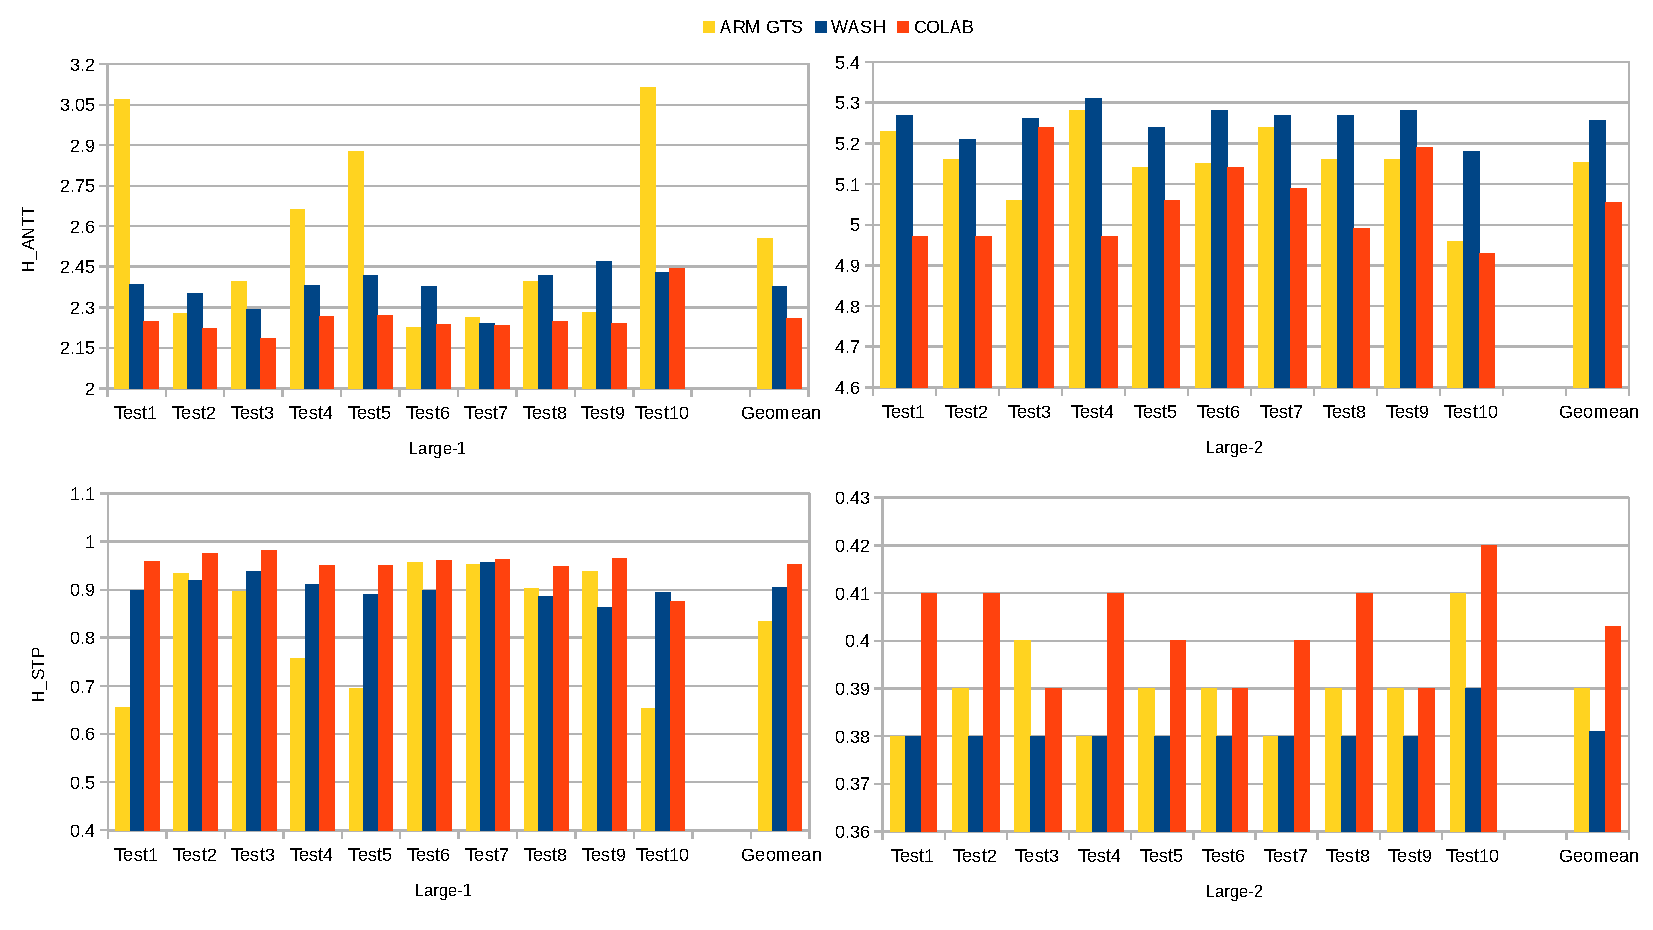
\includegraphics[scale=0.6]{figures/1b1s.pdf}
\caption{Performance of the Large-1 (radix+ocean\_cp) and the Large-2 (ferret+swaptions) workloads using 1 Cortex-A73 core and 1 Cortex-A53 core. Detailed original results from 10 tests with the same 1b1s configuration are presented to show performance variance of ARM GTS scheduler on the real chip. Lower is better for H\_ANTT and higher is better for H\_STP.}
\label{1b1s}
\end{figure*}

\begin{figure}
\centering
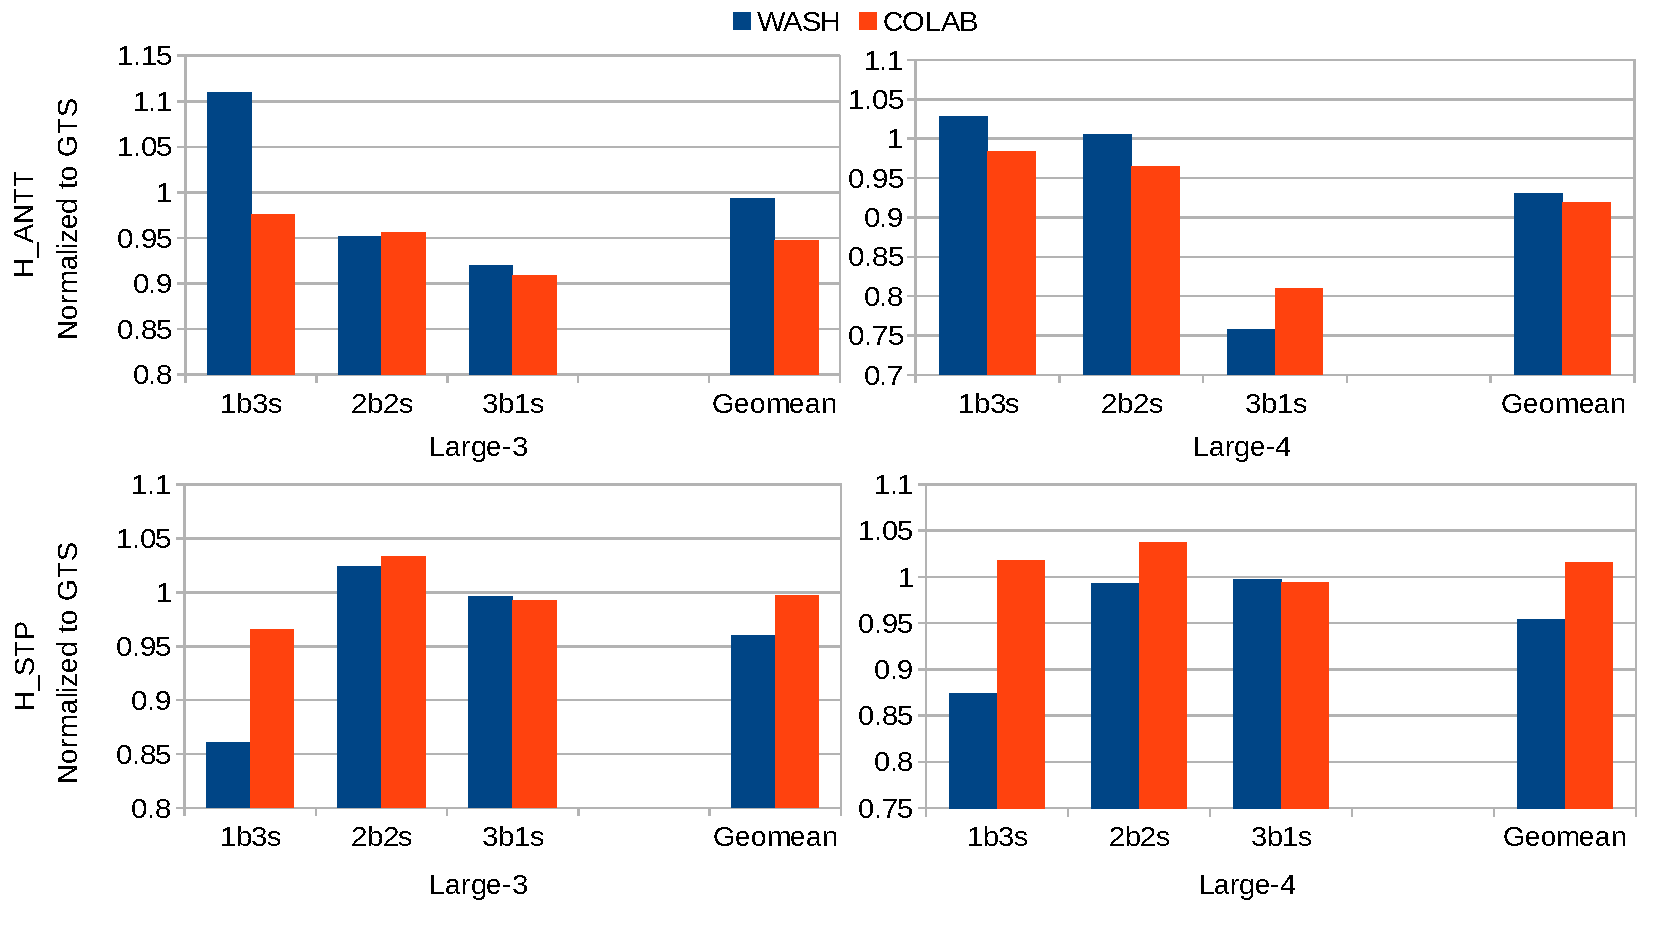
\includegraphics[scale=0.32]{figures/4core.pdf}
\caption{Performance of Large-3 (blackscholes + radix + fluidanimate + water\_spatial) and Large-4 (ocean\_cp + ferret + lu\_cb + swaptions) Workloads using different 4-core configurations. All results are normalized to the ARM GTS ones. Lower is better for H\_ANTT and higher is better for H\_STP.}
\label{4core}
\end{figure}

\begin{figure}
\centering
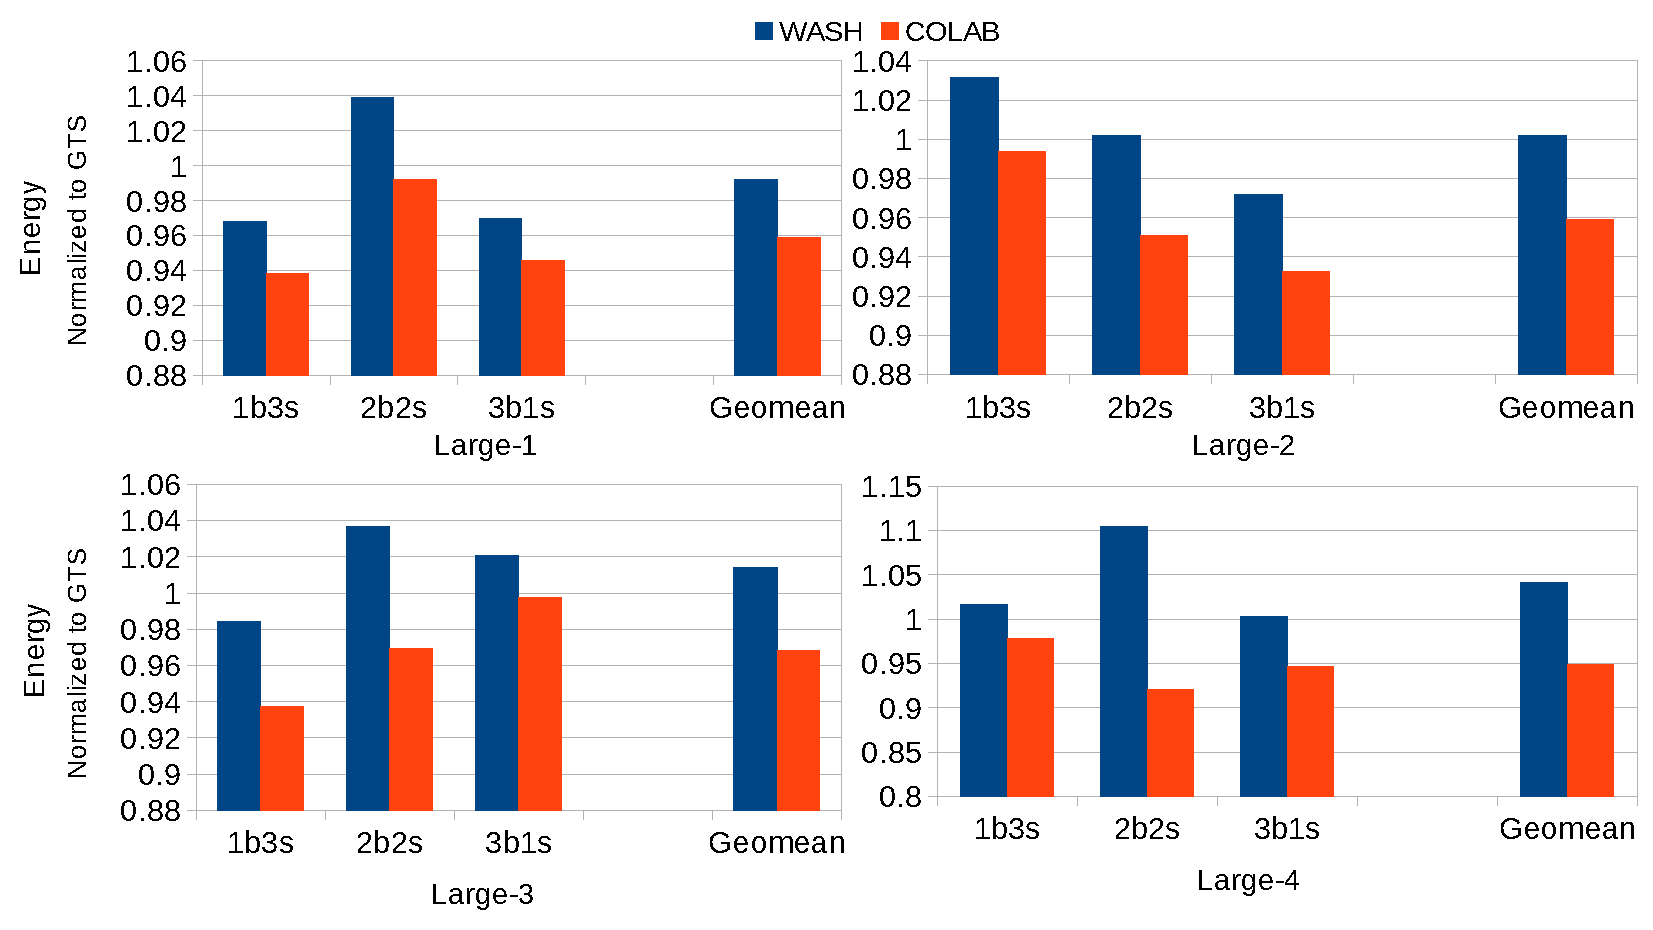
\includegraphics[scale=0.32]{figures/energy_eva.pdf}
\caption{Energy consumption of large multi-programmed Workloads using different 4-core configurations. All results are normalized to the ARM GTS ones. Lower is better for energy.}
\label{elarge}
\end{figure}

\subsection{Experiments on HiHope Hikey 970}
In this section, we validate the performance and the energy efficiency of COLAB with energy-aware extension under large ($simlarge$) mixed multi-threaded multi-programmed workloads on the real ARM big.LITTLE architecture using a HiHope Hikey 970 development board. 
%There is only 4 big cores and 4 little cores in total in the chip. Because we need the baseline performance produced by the fully-big-core configuration, we can only experiment under 2B2S configuration on this development board. The each experiment on real board only take several seconds for $simlarge$ inputs, we can test much large workloads on the board compared with simulation. 

\textbf{\textit{Portable performance on large mixed workloads:}}
Performance variance is significant under the default Linux scheduler (with ARM GTS enable) on the real board compared to checkpoint-based GEM5 simulation. CFS-based ARM GTS scheduler without a core sensitivity aware technique might randomly allocate a high big core speedup thread on either a  big core or a little core.  While WASH and COLAB could make their intelligent decisions if there is a detected high big core speedup thread during runtime. To validate this portable performance, we report performance from 10 tests on two distinct large workloads using a basic 1B1S configuration and then the give the Geo-mean result. 

As shown in the left hand side of Figure~\ref{1b1s}, H\_ANTT results on the Large-1 (radix+ocean\_cp) worklaod for ARM GTS are variant significantly from 2.2 (Test5) to 3.1 (Test10). While for both WASH and COLAB, the H\_ANTT results keep between 2.15 and 2.45. Similar with the results for H\_STP. The Large-1 is a representative mixed workload compared by a high core sensitivity program, ocean\_cp and a low core sensitivity program, radix. The actual speedup between big and little core for ocean\_cp is more than 5x as validated in the performance modelling section. So if ARM GTS unfortunately allocates the high big core speedup threads from ocean\_cp onto the little (Test1, Test4, Test5 and Test10) during execution, COLAB will result in a up-to 27\% (Test10) performance gain compared to ARM GTS. In average, COLAB results in 12\% and 14\% performance gain on H\_ANTT and H\_STP compared to ARM GTS, respectively. WASH can also make kinds of intelligent decisions on keeping the high big core speedup threads from ocean\_cp on the big core. But it will also schedule bottleneck threads from radix, which do not have a good speedup, to occupy the limited big core resources. As a result, COLAB can outperform WASH with an average 5\% performance gain in this workload.

While the main problem of WASH appears when the workload is not core sensitivity as shown in the right hand side of Figre~\ref{1b1s}. Large-2 workload is composed by ferret and swaptions, application threads from both of them don't have significant speedup between big cores and little cores. While, ferret is a synchronization-intensive parallel program which means there will be bottleneck threads during runtime. WASH simply schedules these bottleneck threads to accumulate runqueue of the big core, which can not actually achieve acceleration but make additional system overhead. COLAB shows its unique advantage in this case by in-place accelerate the bottleneck threads on local cores. As a result, COLAB achieves a up-to 6\% (2\% in average) performance gain while WASH suffers a up-to 4.5\% (2\% in average) slowdown on H\_ANTT compared to ARM GTS. The difference is larger for H\_STP, where COLAB achieves a up-to 8\% (3\% in average) performance gain while WASH suffers a up-to 5\% (2\% in average) slowdown compared to ARM GTS.

To further validate the performance of COLAB on general cases, we test two larger workloads (Large-3, Large-4) each composed by 4 programs using distinct 4-core configurations (1B3S, 2B2S and 3B1S). The results are shown in Figure~\ref{4core}, where each bar is the average value of multiple tests by a certain configuration. Similar with the results from GEM5 simulation, COLAB shows its best advantage against WASH on limited big core resource (1B3S). When there is only 1 big core, the bottleneck in-place acceleration technique of COLAB make its intelligent decisions and results in a up-to 12\% (Large-3) performance gain on H\_ANTT compared with WASH. When there are more big core resources, both WASH and COLAB show more advantage as there will be more opportunities to accelerate the needed threads on big cores under core sensitivity aware solutions than CFS-based ARM GTS. For example, WASH and COLAB achieve 24\% and 20\% performance gain on H\_ANTT when running Large-4 on 3B1S configuration compared to ARM GTS. WASH even do better than COLAB as the amount of big cores is sufficient to accelerate both the high speedup and bottleneck threads for the given workload. In average, COLAB achieves 5\%-9\% and 3\%-6\% performance gain on H\_ANTT on the large workloads compared to ARM GTS and WASH, respectively. WASH can not outperform ARM GTS on H\_STP in average based on the problematic scheduling decisions on the 1B3S configuration, while COLAB can still keep good performance.

\textbf{\textit{Energy efficiency on large mixed workloads:}}
%We first test the original COLAB scheduler compared with WASH for performance validation. Then we test the energy-aware COLAB extension for both performance and energy consumption. The default scheduler on the HiHope Hikey 970 board is ARM GTS instead of Linux CFS.
%Figure~\ref{1b1s} shows the performance for these large workloads scheduled by COLAB and WASH against ARM GTS.
Figure~\ref{elarge} shows the performance energy consumption results for large workloads scheduled by COLAB extension and WASH against ARM GTS. In Figure~\ref{elarge}, WASH shows up-to 5\%(Large-4) energy cost. When allocating tasks, WASH simply schedules bottleneck threads to the big core, regardless of how much energy they consume. An application might cost more energy when running in the big core. For ARM GTS, it cannot be aware of energy consumption of tasks. So its result is not very stable and in some cases (Large-1 2B2S and Large-2 1B3S), ARM GTS can outperform WASH with nearly 2\%. 
However, the energy-aware COLAB scheduler takes the advantages of its energy model, uses the predicted energy and allocates each application to proper cores to decrease the consumption. For example, with 1B3S configure, WASH tries to allocate tasks to the big core, which makes the full use of it. But it cost more energy because many tasks are pushed into the run queue of big core. For COLAB, it makes more intelligent decision by considering the energy consumption and schedule those energy-intensive task to little cores in order to reduce the energy consumption.

As shown in Figure-\ref{elarge}, COLAB outperforms ARM GTS and WASH with an average 5\% (up-to 8\%) energy saving in all the large mixed multi-programmed workloads on distinct 4-core based configurations.

%\ty{Figure~\ref{elarge} shows the energy consumption results for these large workloads scheduled by COLAB extension and WASH against ARM GTS.}

%\textbf{\textit{Summary of Experiments:}} Our experiments showed that the state-of-the-art heterogeneous-aware WASH scheduler struggles to make better scheduling decisions that the Linux schedules for synchronization-intensive workloads, computation-intensive workloads, low threads number workloads, high program number workloads, mixed multi-class workloads and limited big cores configurations. Trying to handle both core sensitivity, bottleneck acceleration and fairness through thread affinity alone may lead to too many threads assigned to big cores. Instead, we assign on big cores only threads which run significantly faster on them and we prioritize running bottleneck threads regardless of their thread affinity. This leads to improved turnaround time, higher throughput, and better use of the processor resources compared to both Linux and WASH. In summary from all 312 experiments, COLAB improves turnaround time and system throughput by 11\% and 15\% compared to Linux and by 5\% and 6\% compared to WASH. \vspace{-1em}
%COLAB improves performance by up to 25\% and 21\% lower trunaround time, 11\% and 5\% on average, compared to Linux CFS and WASH scheduler.


%\begin{table*}
 % \caption{Workloads Compositions}
 % \center
 % \label{WC}
 %  \scalebox{0.9}{
 %  \begin{tabular}{p{1.5cm} |p{5.5cm} || p{1.5cm} |p{9cm} }
 %    \toprule[1pt]
 %    \multicolumn{4}{c}{Random-mixed Workloads from PARSEC3.0 and SPLASH-2}\\
 %    \toprule[1pt] 
 %   2B-1 &blackshcoles - radix &4B-1 &blackshcoles - bodytrack - radix - lu\_ncb\\
 %   2B-2 &fft - swaptions &4B-2 &water\_spatial - fmm - fft - fluidanimate\\
 %   2B-3 &lu\_cb - dedup  &4B-3 &lu\_cb - water\_nsquared - fmm - freqmine\\
 %   2B-4 &lu\_ncb - bodytrack &4B-4 &lu\_cb - lu\_ncb - bodytrack - dedup\\
 %  2B-5 &ferret - fluidanimate &4B-5 &radix - lu\_ncb - lu\_cb - fft\\
  %  2B-6 &freqmine - water\_nsquared &4B-6 &blackscholes - bodytrack - dedup - fluidanimate\\
  %  2B-7 &ocean\_cp - fft &4B-7 &radix - ocean\_cp - blackscholes - swaptions\\
  %  2B-8 &ferret - water\_spatial &4B-8 &water\_spatial - water\_nsquared - ferret - freqmine\\
  %  2B-9 &fluidanmiate - fmm &4B-9 &fmm - water\_spatial - ferret - swaptions\\
  %  2B-10 &fmm - water\_spatial &4B-10 &ocean\_cp - fft - fluidanimate - swaptions\\
  %  6B-M &blackshcoles,bodytrack,dedup,radix,lu\_ncb,lu\_cb\\
  %  8B-M &blackshcoles,bodytrack,dedup,fluidanmiate,radix,lu\_ncb,lu\_cb,radiosity\\
  %  12B-M &blackshcoles,bodytrack,dedup,fluidanmiate,streamcluster,swaptions,radix,lu\_ncb,lu\_cb,radiosity,ocean\_cp,fft\\    
%     \midrule
 %    \toprule[1pt]
 %    \multicolumn{4}{c}{Multi/Single-thread multiprogrammed Workloads from PARSEC3.0, SPLASH-2 and SPEC2006}\\
 %    \toprule[1pt]  
 %   3B-1 &blackshcoles - radix - mcf &6B-1 &blackshcoles - bodytrack - radix - lu\_ncb - mcf - bzip2\\
  %  3B-2 &fft - swaptions - mcf &6B-2 &fft - radix - blackscholes - fluidanimate - mcf - bzip2\\
   % 3B-3 &freqmine - swaptions - mcf &6B-3 &blackscholes - dedup - freqmine - swaptions - mcf - bzip2\\
%    3B-4 &blackscholes - freqmine - bzip2 &6B-4 &lu\_cb - lu\_ncb - bodytrack - dedup - mcf - bzip2\\
    %3B-5 &ocean\_cp - fluidanimate - mcf &6B-5 &radix - lu\_ncb - lu\_cb - fft - mcf - bzip2\\
 %   3B-5 &radix - lu\_ncb - bzip2 &6B-5 &radix - lu\_ncb - lu\_cb - fft - mcf - bzip2\\
  %  3B-6 &fluidanimate - freqmine - bzip2 &6B-6 &blackscholes - freqmine - swaptions - fluidanimate - mcf - bzip2\\
   % 3B-7 &blackscholes - fluidanimate - bzip2 &6B-7 &lu\_ncb - ocean\_cp - bodytrack - swaptions - mcf - bzip2\\
%    3B-8 &dedup - fluidanimate - bzip2 &6B-8 &lu\_cb - ocean\_cp - dedup - swaptions - mcf - bzip2\\
 %   3B-9 &lu\_cb - swaptions - bzip2 &6B-9 &ocean\_cp - fft - fluidanimate - swaptions - mcf - bzip2\\
 %   7B-MS   &blackshcoles,bodytrack,dedup,radix,lu\_ncb,lu\_cb,mcf\\
 %   11B-MS &blackshcoles,bodytrack,dedup,canneal,swaptions,radix,lu\_ncb,lu\_cb,radiosity, bzip2,mcf\\ 
  %  15B-MS &blackshcoles,bodytrack,dedup,fluidanmiate,streamcluster,canneal,swaptions,radix,lu\_ncb,lu\_cb,radiosity, ocean\_cp,fft,bzip2,mcf\\   
  % &6B-7 &radix - ocean\_cp - blackscholes - swaptions - mcf - bzip2\\
 %   \bottomrule
 % \end{tabular}}
%\end{table*}
